\documentclass[border=3pt,tikz]{standalone}
\pgfdeclarelayer{bg}% background layer
\pgfsetlayers{bg,main}% order of the layers

\begin{document}

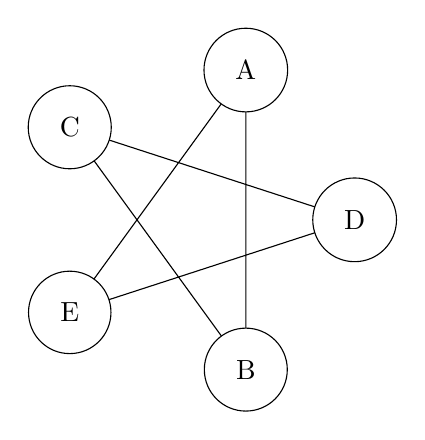
\begin{tikzpicture}

  % draw vertices with nodes
  \foreach [count=\n] \x in {0,...,4} {
    \coordinate (\n) at (-\x*360/5:2);
  };

  % draw vertices with nodes
  \foreach [count=\n] \y in {D,B,E,C,A} {
    \node[shape=circle,draw=black,fill=white,inner sep=2.5mm] at (\n){\y};
  };
  
  \begin{pgfonlayer}{bg}
  \draw (1) -- (4) -- (2) -- (5) -- (3) -- (1);
  \end{pgfonlayer}

  %\draw (1) arc (0:360:2); % draw circle for debugging at coordinate (1) 
  
\end{tikzpicture}


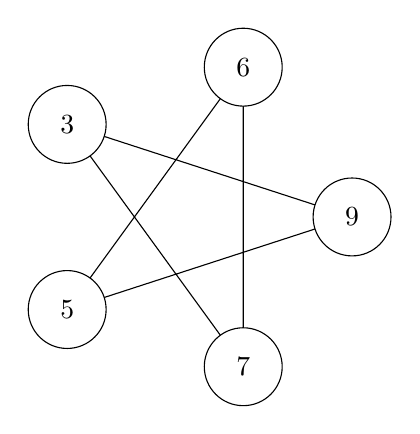
\begin{tikzpicture}

  % draw vertices with nodes
  \foreach [count=\n] \x in {0,...,4} {
    \coordinate (\n) at (-\x*360/5:2);
  };

  % draw vertices with nodes
  \foreach [count=\n] \y in {9,7,5,3,6} {
    \node[shape=circle,draw=black,fill=white,inner sep=2.5mm] at (\n){\y};
  };
  
  \begin{pgfonlayer}{bg}
  \draw (1) -- (4) -- (2) -- (5) -- (3) -- (1);
  \end{pgfonlayer}

\end{tikzpicture}

\end{document}
